% ================================================================================
%
% Copyright (c) 2009--2011, Nico Schlömer
% All rights reserved.
% 
% Redistribution and use in source and binary forms, with or without
% modification, are permitted provided that the following conditions are
% met:
% 
%     * Redistributions of source code must retain the above copyright
%       notice, this list of conditions and the following disclaimer.
%     * Redistributions in binary form must reproduce the above copyright
%       notice, this list of conditions and the following disclaimer in
%       the documentation and/or other materials provided with the distribution
% 
% THIS SOFTWARE IS PROVIDED BY THE COPYRIGHT HOLDERS AND CONTRIBUTORS "AS IS"
% AND ANY EXPRESS OR IMPLIED WARRANTIES, INCLUDING, BUT NOT LIMITED TO, THE
% IMPLIED WARRANTIES OF MERCHANTABILITY AND FITNESS FOR A PARTICULAR PURPOSE
% ARE DISCLAIMED. IN NO EVENT SHALL THE COPYRIGHT OWNER OR CONTRIBUTORS BE
% LIABLE FOR ANY DIRECT, INDIRECT, INCIDENTAL, SPECIAL, EXEMPLARY, OR
% CONSEQUENTIAL DAMAGES (INCLUDING, BUT NOT LIMITED TO, PROCUREMENT OF
% SUBSTITUTE GOODS OR SERVICES; LOSS OF USE, DATA, OR PROFITS; OR BUSINESS
% INTERRUPTION) HOWEVER CAUSED AND ON ANY THEORY OF LIABILITY, WHETHER IN
% CONTRACT, STRICT LIABILITY, OR TORT (INCLUDING NEGLIGENCE OR OTHERWISE)
% ARISING IN ANY WAY OUT OF THE USE OF THIS SOFTWARE, EVEN IF ADVISED OF THE
% POSSIBILITY OF SUCH DAMAGE.
%
% ================================================================================
% ================================================================================
%
% Copyright (c) 2009, Nico Schlömer
% All rights reserved.
% 
% Redistribution and use in source and binary forms, with or without
% modification, are permitted provided that the following conditions are
% met:
% 
%     * Redistributions of source code must retain the above copyright
%       notice, this list of conditions and the following disclaimer.
%     * Redistributions in binary form must reproduce the above copyright
%       notice, this list of conditions and the following disclaimer in
%       the documentation and/or other materials provided with the distribution
% 
% THIS SOFTWARE IS PROVIDED BY THE COPYRIGHT HOLDERS AND CONTRIBUTORS "AS IS"
% AND ANY EXPRESS OR IMPLIED WARRANTIES, INCLUDING, BUT NOT LIMITED TO, THE
% IMPLIED WARRANTIES OF MERCHANTABILITY AND FITNESS FOR A PARTICULAR PURPOSE
% ARE DISCLAIMED. IN NO EVENT SHALL THE COPYRIGHT OWNER OR CONTRIBUTORS BE
% LIABLE FOR ANY DIRECT, INDIRECT, INCIDENTAL, SPECIAL, EXEMPLARY, OR
% CONSEQUENTIAL DAMAGES (INCLUDING, BUT NOT LIMITED TO, PROCUREMENT OF
% SUBSTITUTE GOODS OR SERVICES; LOSS OF USE, DATA, OR PROFITS; OR BUSINESS
% INTERRUPTION) HOWEVER CAUSED AND ON ANY THEORY OF LIABILITY, WHETHER IN
% CONTRACT, STRICT LIABILITY, OR TORT (INCLUDING NEGLIGENCE OR OTHERWISE)
% ARISING IN ANY WAY OUT OF THE USE OF THIS SOFTWARE, EVEN IF ADVISED OF THE
% POSSIBILITY OF SUCH DAMAGE.
%
% ================================================================================

% common header for all exercise sheets
\documentclass[%
paper=a4,
parskip=half,
oneside,
bibliography=totoc
]{scrartcl}

% don't number subsections and deeper
\setcounter{secnumdepth}{1}

% \usepackage{amsbsy,amsmath,amsthm,amsfonts,amssymb,color,xcolor}
\usepackage{amsthm}
\usepackage{graphicx}

% use the latin modern fonts and a better encoding
\usepackage[T1]{fontenc}
\usepackage{lmodern}

% get the fine points of typography
\usepackage{microtype}

\usepackage{math-abbreviations}

% \titlehead{\includegraphics[width=3cm]{../../logos/logo}}
% \subject{\matlab{} in numerical analysis}
\title{Guidelines for writing clean and fast code in \matlab{}}

\author{Nico Schl\"omer\thanks{Universiteit Antwerpen, Middelheimlaan 1, 2020 Antwerpen, Belgium. E-mail: \href{mailto:nico.schloemer@ua.ac.be}{\nolinkurl{nico.schloemer@ua.ac.be}}.}}
\date{\today}
% \publishers{publishers}

\usepackage{listings}  % include highlighted source code
\lstset{% general command to set parameter(s)
basicstyle=\ttfamily,
keywordstyle=\color{matlabeditorkeyword},
identifierstyle=,
commentstyle=\color{matlabeditorcomment},
stringstyle=\color{matlabeditorstring},
showstringspaces=false,     % no special string spaces
frame=single,
language=Matlab,
showlines=true, % don't suppress empty lines
captionpos=b,
abovecaptionskip=2ex
}

\usepackage{subfig}

\usepackage{graphicx}

% have text float around images
\usepackage{floatflt}

\usepackage{tikz}

\usepackage{booktabs}

\theoremstyle{plain}
% \theoremstyle{definition}
\newtheorem*{remark}{Remark}
\newtheorem*{example}{Example}

\usepackage[
bookmarks,
colorlinks=false,
pdftitle={Guidelines for writing clean and fast code in MATLAB(R)},
pdfauthor={Nico Schl\"omer}
]{hyperref}

% get advanced citing capabilities and cite by number
% \usepackage[numbers]{natbib}
% \bibliographystyle{plainnat}
\usepackage[%
bibtex8=true,
hyperref=auto
]{biblatex}
\bibliography{bibtex/matlab-tipsntricks}


\usepackage{marvosym}
\newcommand\cleansymbol{\AtSixty}
\newcommand\fastsymbol{\Lightning}

\newcommand\matlab{\mbox{MATLAB\textsuperscript{\textregistered}}}

% get the euro symbol
\usepackage{eurosym}

% get the trademark symbol correct
\usepackage{textcomp}

\usepackage{siunitx}
\sisetup{obeyall}
\newcommand\extime[1]{\textbf{\SI{#1}{\second}}}

% declare colors
\usepackage{xcolor}
% \definecolor{goodgreen}{cmyk}{1,0,1,0}
\definecolor{goodgreen}{cmyk}{0.8,  0,1,0}
\definecolor{mediocre} {cmyk}{  0,  0,1,0.1}
\definecolor{badred}   {cmyk}{  0,  1,1,0}
% \definecolor{myblue}   {cmyk}{1,1,0,0}
% \definecolor{matlabeditorcomment}{cmyk}{0.87,0.45,0.87,0}
\definecolor{matlabeditorcomment}{RGB}{34,139,34}
\definecolor{matlabeditorkeyword}{RGB}{0,0,255}
\definecolor{matlabeditorstring} {RGB}{181,81,243}


%\usepackage[boxed]{algorithm2e} % pretty-print pseudo code
%\restylealgo{boxed}\linesnumbered\dontprintsemicolon
%\setalcapskip{2ex}
%\renewcommand{\listalgorithmcfname}{Lijst van algoritmen}%
%\renewcommand{\algorithmcfname}{Algoritme}%

\DeclareMathOperator{\diag}{diag}

%\renewcommand{\norm}[1]{\ensuremath{\left\|#1\right\|}}
% \providecommand{\der}[2]{\frac{\partial #1}{\partial #2}}
% \providecommand{\dertwo}[2]{\frac{\partial^2 #1}{\partial #2^2}}


\begin{document}

\maketitle

\begin{abstract}
This document is aimed at \matlab{} beginners who already know the syntax but feel are not yet quite experienced with it. Its goal is to give a number of hints which enable the reader to write quality \matlab{} programs and to avoid commonly made mistakes.

There are three major independent chapters which may very well be read separately. Also, the individual chapters each split up into one or two handful of chunks of information. In that sense, this document is really a slightly extended list of dos and don'ts.

Chapter 1 describes some aspects of \emph{clean} code. The impact of a subsection for the cleanliness of the code is indicated by one to five \cleansymbol--symbols, where five \cleansymbol's want to say that following the given suggestion is of great importance for the comprehensibility of the code.

Chapter 2 describes how to speed up the code and is largely a list of mistakes that beginners may tend to make. This time, the \fastsymbol-symbol represents the amount of speed that you could gain when sticking to the hints given in the respective section.

This guide is written as part of a basic course in numerical analysis, most examples and codes will hence tend to refer to numerical integration or differential equations. However, almost all aspects are of general nature and will also be of interest to anyone using \matlab{}.
\end{abstract}

\tableofcontents


% =============================================================================
%
% Copyright (c) 2009--2013, Nico Schlömer
% All rights reserved.
%
% Redistribution and use in source and binary forms, with or without
% modification, are permitted provided that the following conditions are
% met:
%
%     * Redistributions of source code must retain the above copyright
%       notice, this list of conditions and the following disclaimer.
%     * Redistributions in binary form must reproduce the above copyright
%       notice, this list of conditions and the following disclaimer in
%       the documentation and/or other materials provided with the distribution
%
% THIS SOFTWARE IS PROVIDED BY THE COPYRIGHT HOLDERS AND CONTRIBUTORS "AS IS"
% AND ANY EXPRESS OR IMPLIED WARRANTIES, INCLUDING, BUT NOT LIMITED TO, THE
% IMPLIED WARRANTIES OF MERCHANTABILITY AND FITNESS FOR A PARTICULAR PURPOSE
% ARE DISCLAIMED. IN NO EVENT SHALL THE COPYRIGHT OWNER OR CONTRIBUTORS BE
% LIABLE FOR ANY DIRECT, INDIRECT, INCIDENTAL, SPECIAL, EXEMPLARY, OR
% CONSEQUENTIAL DAMAGES (INCLUDING, BUT NOT LIMITED TO, PROCUREMENT OF
% SUBSTITUTE GOODS OR SERVICES; LOSS OF USE, DATA, OR PROFITS; OR BUSINESS
% INTERRUPTION) HOWEVER CAUSED AND ON ANY THEORY OF LIABILITY, WHETHER IN
% CONTRACT, STRICT LIABILITY, OR TORT (INCLUDING NEGLIGENCE OR OTHERWISE)
% ARISING IN ANY WAY OUT OF THE USE OF THIS SOFTWARE, EVEN IF ADVISED OF THE
% POSSIBILITY OF SUCH DAMAGE.
%
% =============================================================================
\newpage
\section*{\matlab{} alternatives}
\addcontentsline{toc}{section}{\matlab{} alternatives}

When writing \matlab{} code, you need to realize that unlike C, Fortran, or
Python code, you will always need the \emph{commercial} \matlab{} environment
to have it run. Right now, that might not be much of a problem to you as you
are at a university or have some other free access to the software, but
sometime in the future, this might change.

The current cost for the basic \matlab{} kit, which does not include
\emph{any} toolbox nor Simulink, is \EUR{500} for academic institutions;
around \EUR{60} for students; \emph{thousands} of Euros for commercial
operations. Considering this, there is a not too small chance that you will
not be able to use \matlab{} after you quit from university, and that would
render all of your own code virtually useless to you.

Because of that, free and open source \matlab{} alternatives have emerged,
three of which are shortly introduced here. Octave and Scilab try to stick to
\matlab{} syntax as closely as possible, resulting in all of the code in this
document being legal for the two packages as well.  When it comes to the
specialized toolboxes, however, neither of the alternatives may be able to
provide the same capabilities that \matlab{} offers. However, these are mostly
functions related to Simulink and the like which are hardly used by beginners
anyway.  Also note none of the alternatives ships with its own text editor (as
\matlab{} does), so you are free yo use the editor of your choice (see, for
example, \href{http://www.vim.org/}{vim},
\href{http://www.gnu.org/software/emacs/}{emacs}, Kate,
\href{http://projects.gnome.org/gedit/}{gedit} for Linux;
\href{http://notepad-plus.sourceforge.net/uk/site.htm}{Notepad++},
\href{http://www.crimsoneditor.com/}{Crimson Editor} for Windows).

\subsection{Python}

\begin{floatingfigure}[r]{6cm}
\centering

\includegraphics[width=6cm]{figures/python-logo-generic}
\end{floatingfigure}

Python is the most modern programming language as of 2013: Amongst the many
award the language as received stands the TIOBE Programming Language Award of
2010. It is yearly given to the programming language that has gained the
largest market market share during that year.

Python is used in all kinds of different contexts, and its versatility and
ease of use has made it attractive to many. There are tons packages for all
sorts of tasks, and the huge community and its open development help the
enormous success of Python.

In the world of scientific computing, too, Python has already risen to be a
major player. This is mostly due to the packages SciPy and Numpy which provide
all data structures and algorithms that are used in numerical code. Plotting
is most easily handled by matplotlib, a huge library which in many ways excels
\matlab{}'s graphical engine.

Being a language rather than an application, Python is supported in virtually
every operating system.

The author of this document highly recommends to take a look at Python for
your own (scientific) programming projects.


\subsection{GNU Octave}

\begin{floatingfigure}[r]{5cm}
\centering
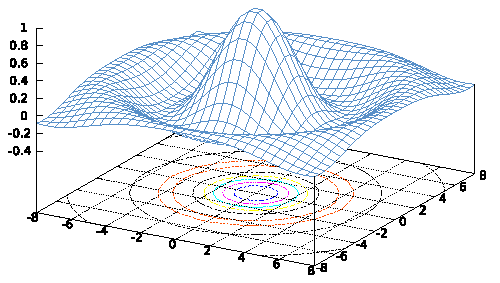
\includegraphics[width=5cm]{figures/Octave_Sombrero}
\end{floatingfigure}

GNU Octave is a high-level language, primarily intended for numerical
computations. It provides a convenient command line interface for solving
linear and nonlinear problems numerically, and for performing other numerical
experiments using a language that is mostly compatible with \matlab{}. It may
also be used as a batch-oriented language.

Internally, Octave relies on other independent and well-recognized packages
such as gnuplot (for plotting) or UMFPACK (for calculating with sparse
matrices). In that sense, Octave is extremely well integrated into the free
and open source software (FOSS) landscape.

Octave has extensive tools for solving common numerical linear algebra
problems, finding the roots of nonlinear equations, integrating ordinary
functions, manipulating polynomials, and integrating ordinary differential and
differential-algebraic equations. It is easily extensible and customizable via
user-defined functions written in Octave's own language, or using dynamically
loaded modules written in C++, C, Fortran, or other languages.

GNU Octave is also freely redistributable software. You may redistribute it
and/or modify it under the terms of the GNU General Public License (GPL) as
published by the Free Software Foundation.

The project if originally GNU/Linux, but versions for MacOS, Windows, Sun
Solaris, and OS/2 exist.

\subsection{Scilab}

\begin{floatingfigure}[r]{4cm}
\centering

\includegraphics[width=4cm]{figures/scilab_official_logo}
\end{floatingfigure}

Scilab is a scientific software package for numerical computations providing a
powerful open computing environment for engineering and scientific
applications.

Scilab is open source software and originates from the French International
Institute for Research in Computer Science and Control (INRIA).

Since 1994 it has been distributed freely along with the source code via the
Internet. It is currently used in educational and industrial environments
around the world.

Scilab is now the responsibility of the Scilab Consortium, launched in May
2003. There are currently 18 members in Scilab Consortium (Phase II).

Scilab includes hundreds of mathematical functions with the possibility to add
interactively programs from various languages (C, C++, Fortran,\dots). It has
sophisticated data structures (including lists, polynomials, rational
functions, linear systems\dots), an interpreter and a high level programming
language.

Scilab works under Windows 9X/2000/XP/Vista, GNU/Linux, and most UNIX systems.
Binary versions for these systems are freely available, along with the source
code.

\subsection{Julia}

Quoting from \url{julialang.org}:\\
\begin{wrapfigure}{r}{4cm}
  \centering
  
\includegraphics[width=4cm]{figures/julia.png}
\end{wrapfigure}
%\begin{floatingfigure}[r]{4cm}
%  \centering
%  
\includegraphics[width=4cm]{figures/julia.png}
%\end{floatingfigure}
\begin{quote}
Julia is a high-level, high-performance dynamic programming language for
technical computing, with syntax that is familiar to users of other technical
computing environments. It provides a sophisticated compiler, distributed
parallel execution, numerical accuracy, and an extensive mathematical function
library. The library, largely written in Julia itself, also integrates mature,
best-of-breed C and Fortran libraries for linear algebra, random number
generation, signal processing, and string processing. In addition, the Julia
developer community is contributing a number of external packages through
Julia’s built-in package manager at a rapid pace. IJulia, a collaboration
between the IPython and Julia communities, provides a powerful browser-based
graphical notebook interface to Julia.
\end{quote}

% ================================================================================
%
% Copyright (c) 2009, Nico Schlömer
% All rights reserved.
% 
% Redistribution and use in source and binary forms, with or without
% modification, are permitted provided that the following conditions are
% met:
% 
%     * Redistributions of source code must retain the above copyright
%       notice, this list of conditions and the following disclaimer.
%     * Redistributions in binary form must reproduce the above copyright
%       notice, this list of conditions and the following disclaimer in
%       the documentation and/or other materials provided with the distribution
% 
% THIS SOFTWARE IS PROVIDED BY THE COPYRIGHT HOLDERS AND CONTRIBUTORS "AS IS"
% AND ANY EXPRESS OR IMPLIED WARRANTIES, INCLUDING, BUT NOT LIMITED TO, THE
% IMPLIED WARRANTIES OF MERCHANTABILITY AND FITNESS FOR A PARTICULAR PURPOSE
% ARE DISCLAIMED. IN NO EVENT SHALL THE COPYRIGHT OWNER OR CONTRIBUTORS BE
% LIABLE FOR ANY DIRECT, INDIRECT, INCIDENTAL, SPECIAL, EXEMPLARY, OR
% CONSEQUENTIAL DAMAGES (INCLUDING, BUT NOT LIMITED TO, PROCUREMENT OF
% SUBSTITUTE GOODS OR SERVICES; LOSS OF USE, DATA, OR PROFITS; OR BUSINESS
% INTERRUPTION) HOWEVER CAUSED AND ON ANY THEORY OF LIABILITY, WHETHER IN
% CONTRACT, STRICT LIABILITY, OR TORT (INCLUDING NEGLIGENCE OR OTHERWISE)
% ARISING IN ANY WAY OUT OF THE USE OF THIS SOFTWARE, EVEN IF ADVISED OF THE
% POSSIBILITY OF SUCH DAMAGE.
%
% ================================================================================
\newpage
\section{Coding clean}

There is a plethora of reasons why code that \emph{just works\texttrademark} is not good enough. Take a peek at listing \ref{listing:prime1} and admit:

\begin{itemize}
% maintainability:
\item Fixing bugs, adding features, and working with the code in all other aspects get a lot easier when the code isn't messy.
% readability:
\item Imagine someone else looking at your code, and trying to figure out what it does. In case you have you didn't keep it clean, that will certainly be a huge waste of time.
\item You might be planning to code for a particular purpose now, not planning on ever using it again, but experience tells that there is virtually no computational task that you come across only once in your programming life. Imagine yourself looking at your own code, a week, a month, or a year from now: Would you still be able to understand why the code works as it does? Clean code will make sure you do.
\end{itemize}

Examples of messy, unstructured, and generally ugly programs are plenty, but there are also places where you are almost guaranteed to find well-structured code. Take, for example the \matlab{} internals: Many of the functions that you might make use of when programming \matlab{} are implemented in \matlab{} syntax themselves -- by professional MathWorks programmers. To look at such the contents of the \lstinline!mean()! function (which calculates the average mean value of an array), type \lstinline!edit mean! on the \matlab{} command line. You might not be able to understand what's going on, but the way the file looks like may give you hints on how to write clean code.


\begin{lstlisting}[framerule=2pt,rulecolor=\color{badred},float=b,label={listing:prime1},caption={Perfectly legal \matlab{} code, with all rules of style ignored. Can you guess what this function does?}]
function lll(ll1,l11,l1l);if floor(l11/ll1)<=1;...
lll(ll1,l11+1,l1l );elseif mod(l11,ll1)==0;lll(...
ll1,l11+1,0);elseif mod(l11,ll1)==floor(l11/...
ll1)&&~l1l;floor(l11/ll1),lll(ll1,l11+1,0);elseif...
mod(l11,ll1)>1&&mod(l11,ll1)<floor(l11/ll1),...
lll(ll1,l11+1,l1l+~mod(floor(l11/ll1),mod(l11,ll1)) );
elseif l11<ll1*ll1;lll(ll1,l11+1,l1l);end;end
\end{lstlisting}

\subsection{Multiple functions per file  -- \cleansymbol\cleansymbol\cleansymbol}
It is a common and false prejudice that \matlab{} cannot cope with several functions per file. The truth is: There \emph{may} be more than one function in a file, but just the first one in the file will be \emph{visible} to functions in other files or to the command line. In that sense, those functions in a file which do not take the first position can (only) act as a helper for the function on top (see listing \ref{listing:multiple-functions}).

When writing code, think about whether or not a particular function is really just a helper, or if needs to be allowed to be called from somewhere else. Doing so, you can avoid a cluttered mess of dozens of M-files in your program folder.

\begin{lstlisting}[framerule=2pt,rulecolor=\color{goodgreen},float,label={listing:multiple-functions},caption={One source containing three functions: Useful when \lstinline!helperFun1! and \lstinline!helperFun2! are only needed by \lstinline!topFun!.}]
% ===========================================================
% callable from outside:
function topFun
  % [...]
  % calls helperFun1 and helperFun2
  % [...]
end
% ===========================================================


% ===========================================================
% only visible to all functions in this file:
function helperFun1
  % [...]
end
% ===========================================================


% ===========================================================
% only visible to all functions in this file:
function helperFun2
  % [...]
end
% ===========================================================
\end{lstlisting}


\paragraph{Subfunctions -- \cleansymbol\cleansymbol}
An issue that may come up if you have quite a lot of functions per file might be that you lose sight of which function actually requires which other function.

In case one of the functions is a helper function for not more than one other function, a clean place to put it would be \emph{inside} the other function. This way, it will only be visible to the surrounding function and its name will not interfere with the name of any other subfunction. The biggest advantage, however, is certainly that the subfunction is then syntactically \emph{clearly associated} with its parent function. When 
looking at the code for the first time, the relations between the functions are immediately visible.


\hfill
\begin{minipage}[t]{.45\textwidth}
\begin{lstlisting}[framerule=2pt,rulecolor=\color{badred}]
% [...]

% =========================
function fun1
  % call helpFun1 here
end
% =========================

% =========================
function fun2
  % call helpFun2 here
end
% =========================

% =========================
function helpFun1
   % [...]
end
% =========================

% =========================
function helpFun2
   % [...]
end
% =========================

% [...]
\end{lstlisting}
The routines \lstinline!fun1!, \lstinline!fun2!, \lstinline!helpFun1!, and \lstinline!helpFun2! are sitting next to each other and no hierarchy is visible.
\end{minipage}
\hfill
\begin{minipage}[t]{.45\textwidth}
\begin{lstlisting}[framerule=2pt,rulecolor=\color{goodgreen}]
% [...]

% =========================
function fun1
  % call helpFun here

  % -----------------------
  function helpFun
     % [...]
  end
  % -----------------------
end
% =========================

% =========================
function fun2
  % call helpFun here

  % -----------------------
  function helpFun
     % [...]
  end
  % -----------------------
end
% =========================

% [...]
\end{lstlisting}
Immediately obvious: The first \lstinline!helpFun! helps \lstinline!fun1!, the second \lstinline!fun2! -- and does nothing else.
\end{minipage}
\hfill

% \begin{lstlisting}[framerule=2pt,rulecolor=\color{goodgreen},float,label={listing:multiple-functions},caption={Two function having subfunction with the same name.}]
% 
% \end{lstlisting}




\subsection{Variable and function names -- \cleansymbol\cleansymbol\cleansymbol}

One key ingredient for a consistent source code is a consistent naming scheme for the variables in use. From the dawn of programming languages in the 1950's, schemes have developed and decayed and are generally subject to evolution. There are, however, some general rules which have proven useful over the years in all kinds of various contexts. In \cite{Johnson:2002:MPS}, a crisp and yet comprehensive overview on many aspects of variable naming is given; a few of the most useful ones are stated here.

\paragraph{Variable names tell what the variable does.} Undoubtedly, this is the first and foremost rule in variable naming, and it implies several things.

\begin{itemize}
\item Of course, you wouldn't name a variable \lstinline!pi! when it really holds the value \lstinline!2.718128!, right?
\item In mathematics and computer science, some names are connected to certain meanings. Table \ref{table:typical-variable-usage} lists a number of widely used conventions.

\begin{table}
\centering
\begin{tabular}{ll}
\toprule
Variable name                                                 & Usual purpose\\\midrule
\lstinline!m!, \lstinline!n!                                  & integer sizes (,e.g., the dimension of a matrix)\\
\lstinline!i!, \lstinline!j!, \lstinline!k! (, \lstinline!l!) & integer numbers (mostly loop indices)\\
\lstinline!x!, \lstinline!y!                                  & real values ($x$-, $y$-axis)\\
\lstinline!z!                                                 & complex value or $z$-axis\\
\lstinline!c!                                                 & complex value or constant (or both)\\
\lstinline!t!                                                 & time value\\
\lstinline!e!                                                 & the Eulerian number or `unit' entities\\
\lstinline!f!, \lstinline!g! (, \lstinline!h!)                & generic function names\\
\lstinline!h!                                                 & spatial discretization parameter (in numerical analysis)\\
\lstinline!epsilon!, \lstinline!delta!                        & small real entities\\
\lstinline!alpha!, \lstinline!beta!                           & angles or parameters\\
\lstinline!theta!, \lstinline!tau!                            & parameters, time discretization parameter (in n.a.)\\
\lstinline!kappa!, \lstinline!sigma!, \lstinline!omega!       & parameters\\
\lstinline!u!, \lstinline!v!, \lstinline!w!                   & vectors\\
\lstinline!A!, \lstinline!M!                                  & matrices\\
\lstinline!b!                                                 & right-hand side of an equation system\\\bottomrule
\end{tabular}
\caption{Variable names and their usual purposes in source codes. These guidelines aren't particularly strict, but for example one would never use \lstinline!i! to hold a float number, nor \lstinline!x! for an integer.}
\label{table:typical-variable-usage}
\end{table}
\end{itemize}

\paragraph{Short variable names.}
Short, non-descriptive variable names are quite common in mathematical computing as the variable names in the corresponding (pen and paper) calculations are hardly ever longer then one character either (see table \ref{table:typical-variable-usage}). To be able to distinguish between vector and matrix entities, it is common practice in programming as well as mathematics to denote matrices by upper-case, vectors and scalars by lower-case characters.

\hfill
\begin{minipage}[t]{.45\textwidth}
\begin{lstlisting}[framerule=2pt,rulecolor=\color{badred}]
K = 20;
a = zeros(K,K);
B = ones(K,1);

U = a*B;
\end{lstlisting}
\end{minipage}
\hfill
\begin{minipage}[t]{.45\textwidth}
\begin{lstlisting}[framerule=2pt,rulecolor=\color{goodgreen}]
k = 20;
A = zeros(k,k);
b = ones(k,1);

u = A*b;
\end{lstlisting}
\end{minipage}
\hfill


\paragraph{Long variable names.}
A widely used convention mostly in the C++ development community to write long, descriptive variables in mixed case starting with lower case, such as
\begin{lstlisting}
linearity, distanceToCircle, figureLabel.
\end{lstlisting}
Alternatively, one could use the underscore to separate parts of a compound variable name:
\begin{lstlisting}
linearity, distance_to_circle, figure_label.
\end{lstlisting}
This technique, although readable, is not commonly used for variable names in other languages. Also, some feel the underscore character is not quite easily typable on the keyboard.

When still using the underscore notation, watch out for variable names in \matlab{}'s plots: its \TeX-interpreter will treat the underscore as a switch to subscript and a variable name such as \lstinline!distance_to_circle! will read \lstinline!distance!$_{\text{\lstinline!t!}}$\lstinline!o!$_{\text{\lstinline!c!}}$\lstinline!ircle! in the plot.

\begin{remark}
Using the hyphen `\lstinline!-!' as a separator cannot be considered: \matlab{} will immediately interpret `\lstinline!-!' as the minus sign, \lstinline!distance-to-circle! is ``\lstinline!distance! minus \lstinline!to! minus \lstinline!circle!''. The same holds for function names.
\end{remark}

% \paragraph{Variables with a large scope should have meaningful names. Variables with a small
% scope can have short names.}
% In practice most variables should have meaningful names. The use of short names should be
% reserved for conditions where they clarify the structure of the statements. Scratch variables used
% for temporary storage or indices can be kept short. A programmer reading such variables should
% be able to assume that its value is not used outside a few lines of code. Common scratch variables
% for integers are i, j, k, m, n and for doubles x, y and z.

\paragraph{Logical variable names.} If a variable is supposed to only hold the values \lstinline!0! or \lstinline!1! to represent \lstinline!true! or \lstinline!false!, then the variable name should express that. A common technique is to prepend the variable name by \lstinline!is! and, less common, by \lstinline!flag!.
\begin{lstlisting}
isPrime, isInside, flagCircle
\end{lstlisting}


\subsection{Indentation -- \cleansymbol\cleansymbol\cleansymbol\cleansymbol}

If you ever dealt with nested \lstinline!for!- and \lstinline!if! constructs, then you probably noticed that it may sometimes be hard to distinguish those nested constructions from other code at first sight. Also, if the contents of a loop extend over more than just a few lines, a visual aid may be helpful for indicating what is inside and what is outside the loop -- and this is where indentation comes into play.

Usually, one would indent everything within a loop, a function, a conditional, a \lstinline!switch! statement and so on. Depending on who you ask, you'll be told to indent by two, three, or four spaces, or one tab. As a general rule, the indentation should yield a clear visual distinction while not using up all your space on the line (see next paragraph).

\hfill
\begin{minipage}[t]{.45\textwidth}
\begin{lstlisting}[framerule=2pt,rulecolor=\color{badred}]
for i=1:n
for j=1:n
if A(i,j)<0
A(i,j) = 0;
end
end
end
\end{lstlisting}
No visual distinction between the loop levels makes it hard to recognize where the first loop ends.\footnotemark
\end{minipage}
\hfill
\begin{minipage}[t]{.45\textwidth}
\begin{lstlisting}[framerule=2pt,rulecolor=\color{goodgreen}]
for i=1:n
    for j=1:n
        if A(i,j)<0
            A(i,j) = 0;
        end
    end
end
\end{lstlisting}
With indentation, the code looks a lot clearer.\footnotemark[\value{footnote}]
\end{minipage}
\hfill

\footnotetext{What the code does is replacing all negative entries of an \lstinline!n!$\times$\lstinline!n!-matrix by \lstinline!0!. There is, however, a much better (shorter, faster) way to achieve this: \lstinline!A( A<0 ) = 0;! (see page \pageref{sec:logicalIndexing}).}





\subsection{Line length -- \cleansymbol}
There is de facto no limit on how much you can write on a single line of \matlab{} code. In fact, you could condense every \matlab{} code to a ``one-liner'' by separating two commands by a `\lstinline!;!' or a `\lstinline!,!', and suppress the newline character between them. However, a single line with one million characters will potentially not be very readable.

But, how many characters can you fit onto a single line without obscuring its content? This is certainly debatable, but commonly this value sits somewhere between 70 and 80; \matlab{}'s own text editor suggests 75 characters per line. This way, one makes also sure that it is not necessary to have a 22" widescreen monitor to be able to display the code without artificial line breaks or horizontal scrolling in the editor.

Sometimes of course your lines need to stretch longer than this, but that's why \matlab{} contains the ellipses `\lstinline!...!' which makes sure the line following the line with the ellipsis is read as if there was no line break at all.

\hfill
\begin{minipage}[t]{.45\textwidth}
\begin{lstlisting}[framerule=2pt,rulecolor=\color{goodgreen}]
a = sin( exp(x) ) ...
  - alpha* 4^6    ...
  + u'*v;
\end{lstlisting}
\end{minipage}
\hfill
\begin{minipage}[t]{.45\textwidth}
\begin{lstlisting}[framerule=2pt,rulecolor=\color{badred}]
a = sin( exp(x) ) - alpha* 4^6 + u'*v;


\end{lstlisting}
\end{minipage}
\hfill


\subsection{Spaces and alignment -- \cleansymbol\cleansymbol\cleansymbol}\label{paragraph:alignment}
In some situations, it makes sense to break a line although it hasn't up to the limit, yet. This may be the case when you are dealing with an expression that -- because of its length -- has to break anyway further to the right; then, one would like to choose the line break point such that it coincides with \emph{semantic} or \emph{syntactic} break in the syntax. For examples, see the code below.

\hfill
\begin{minipage}[t]{.45\textwidth}
\begin{lstlisting}[framerule=2pt,rulecolor=\color{badred}]
A = [ 1, 0.5 , 5; 4, ...
42.23, 33; 0.33, ...
pi, 1];

a = alpha*(u+v)+beta*...
sin(p'*q)-t...
*circleArea(10);
\end{lstlisting}
Unsemantic line breaks decrease the readability. Neither the shape of the matrix, nor the number of summands in the second expression is clear.
\end{minipage}
\hfill
\begin{minipage}[t]{.45\textwidth}
\begin{lstlisting}[framerule=2pt,rulecolor=\color{goodgreen}]
A = [ 1   , 0.5  , 5 ; ...
      4   , 42.23, 33; ...
      0.33, pi   , 1   ];

a = alpha* (u+v)     ...
  + beta*  sin(p'*q) ...
  - t*     circleArea(10);
\end{lstlisting}
The shape and contents of the matrix, as well as the elements of the second expression, are immediately visible to the programmer.
\end{minipage}
\hfill

\paragraph{Spaces in expressions} Closely related to this is the usage of spaces in expressions. The rule is, again: put spaces there where \matlab{}'s syntax would. Consider the following example.

\hfill
\begin{minipage}[t]{.45\textwidth}
\begin{lstlisting}[framerule=2pt,rulecolor=\color{badred}]
aValue = 5+6 / 3*4;
\end{lstlisting}
This spacing suggests that the value of \lstinline!aValue! will be $11/12$, which is of course not the case.
\end{minipage}
\hfill
\begin{minipage}[t]{.45\textwidth}
\begin{lstlisting}[framerule=2pt,rulecolor=\color{goodgreen}]
aValue = 5 + 6/3*4;
\end{lstlisting}
Much better, as the the fact that the addition is executed last gets reflected by according spacing.
\end{minipage}
\hfill



\subsection{Magic numbers -- \cleansymbol\cleansymbol\cleansymbol}

When coding, sometimes you consider a value constant because you do not intend to change it anytime soon. Take, for example, a program that determines whether or not a given point sits outside a circle of radius $1$ with center $(1,1)$ and at the same time inside a square of edge length $2$, right enclosing the circle (see \cite{Hull:2006:CCM}).

When finished, the code will contain a couple of \lstinline!1!'s but it'll not be clear if they are distinct or refer to the same abstract value (see below). Those hardcoded numbers are frequently called \emph{magic numbers}, as they do what they are supposed to do, but one can't easily tell why. When you, after some time, change your mind and you do want to change the value of the radius, it'll be rather difficult to identify those \lstinline!1!'s which actually refer to it.


\hfill
\begin{minipage}[t]{.45\textwidth}\label{example:magic-numbers}
\begin{lstlisting}[framerule=2pt,rulecolor=\color{badred}]
x = 2; y = 0;




pointsDistance = ...
  norm( [x,y]-[1,1] );

isInCircle = ...
      (pointsDistance < 1);
isInSquare = ...
     ( abs(x-1)<1 ) && ...
     ( abs(y-1)<1 );

if ~isInCircle && isInSquare
% [...]
\end{lstlisting}
It is not immediately clear if the various \lstinline!1!'s do in the code and whether or not they represent one entity. These numbers are called \emph{magic numbers}.
\end{minipage}
\hfill
\begin{minipage}[t]{.45\textwidth}
\begin{lstlisting}[framerule=2pt,rulecolor=\color{goodgreen}]
x = 2; y = 0;

radius = 1;
xc = 1; yc = 1;

pointsDistance = ...
  norm( [x,y]-[xc,yc] );

isInCircle = ...
 (pointsDistance < radius);
isInSquare = ...
 ( abs(x-xc)<radius ) && ...
 ( abs(y-yc)<radius );

if ~isInCircle && isInSquare
% [...]
\end{lstlisting}
The meaning of the variable \lstinline!radius! is can be instantly seen and its value easily altered.
\end{minipage}
\hfill


\subsection{Comments  -- \cleansymbol\cleansymbol\cleansymbol\cleansymbol\cleansymbol}

The most valuable character for clean \matlab{} code is `\lstinline!%!',
the comment character. All tokens after it on the same line are ignored, and the space can be used to explain the source code in English (or your tribal language, if you prefer).

\paragraph{Documentation -- \cleansymbol\cleansymbol\cleansymbol\cleansymbol\cleansymbol}
There should be a big fat neon-red blinking frame around this paragraph, as documentation is \emph{the} single most important aspect about clean and readable code. Unfortunately, it also takes the longest to write which is why you will find undocumented source code everywhere you go.

Look at listing \ref{listing:fences} for a suggestion for quick and clear documentation, and see if you can do it yourself!


\paragraph{Structuring elements -- \cleansymbol\cleansymbol\cleansymbol}
It is always useful to have the beginning and the end of the function not only indicated by the respective keywords, but also by something more visible. Consider building `fences' with commented `\lstinline!#!', `\lstinline!=!', or `\lstinline!-!' characters, to visually separate distinct parts of the code. This comes in very handy when there are multiple functions in one source file, for example, or when there is a \lstinline!for!-loop that stretches over that many lines that you can't easily find the corresponding \lstinline!end! anymore.

For a (slightly exaggerated) example, see listing \ref{listing:fences}.

\begin{lstlisting}[float,label={listing:fences},caption={Function in which \lstinline!-!-fences are used to emphasize the functionally separate sections of the code.}]
% ===========================================================
% *** FUNCTION timeIteration
% ***
% *** Takes a starting vector u and performs n time steps.
% ***
% ===========================================================
function out = timeIteration( u, n )

  % ---------------------------------------------------------
  % set the parameters
  tau   = 1.0;
  kappa = 1.0;
  out   = u;
  % ---------------------------------------------------------


  % ---------------------------------------------------------
  % do the iteration
  for k = 1:n

      [out, flag] = proceedStep( out, tau, kappa );

      % - - - - - - - - - - - - - - - - - - - - - - - - - -
      % warn if something went wrong
      if ~flag
          warning( [ 'myProg:timeIteration', ...
                     'proceedStep returns flag ', flag ] );
      end
      % - - - - - - - - - - - - - - - - - - - - - - - - - -

  end
  % ---------------------------------------------------------

end
% ===========================================================
% *** END FUNCTION timeIteration
% ===========================================================
\end{lstlisting}


\subsection{Usage of brackets -- \cleansymbol\cleansymbol}
Of course, there is a clearly defined operator precedence list in \matlab{} (see table \ref{table:operator-precedence}) that makes sure that for every \matlab{} expression, involving any unary or binary operator, there is a unique way of evaluation. It is quite natural to remember that \matlab{} treats multiplication (\lstinline!*!) before addition (\lstinline!+!), but things may get less intuitive when it comes to logical operators, or a mix of numerical and logical ones (although this case is admittedly very rare).

Of course one can always look those up (see table \ref{table:operator-precedence}), but to save the work one could equally quick just insert a pair of bracket at the right spot, although they may be unnecessary -- this will certainly help avoiding confusion.

\hfill
\begin{minipage}[t]{.45\textwidth}
\begin{lstlisting}[framerule=2pt,rulecolor=\color{badred}]
isGood =  a<0 ...
       && b>0 || k~=0;
\end{lstlisting}
Without knowing if \matlab{} first evaluates the short-circuit AND `\lstinline!&&!' or the short-circuit OR `\lstinline!||!', it is impossible to predict the value of \lstinline!isGood!.
\end{minipage}
\hfill
\begin{minipage}[t]{.45\textwidth}
\begin{lstlisting}[framerule=2pt,rulecolor=\color{goodgreen}]
isGood = ( a<0 && b>0 ) ...
       || k~=0;
\end{lstlisting}
With the (unnecessary) brackets, the situation is clear.
\end{minipage}
\hfill


\begin{table}
\begin{enumerate}
\item Parentheses \lstinline!()!
\item Transpose (\lstinline!.'!), power (\lstinline!.^!), complex conjugate transpose (\lstinline!'!), matrix power (\lstinline!^!)
\item Unary plus (\lstinline!+!), unary minus (\lstinline!-!), logical negation (\lstinline!~!)
\item Multiplication (\lstinline!.*!), right division (\lstinline!./!), left division (\lstinline!.\!), matrix multiplication (\lstinline!*!), matrix right division (\lstinline!/!), matrix left division (\lstinline!\!)
\item Addition (\lstinline!+!), subtraction (\lstinline!-!)
\item Colon operator (\lstinline!:!)
\item Less than (\lstinline!<!), less than or equal to (\lstinline!<=!), greater than (\lstinline!>!), greater than or equal to (\lstinline!>=!), equal to (\lstinline!==!), not equal to (\lstinline!~=!)
\item Element-wise AND (\lstinline!&!)
\item Element-wise OR (\lstinline!|!)
\item Short-circuit AND (\lstinline!&&!)
\item Short-circuit OR (\lstinline!||!)
\end{enumerate}
\caption{\matlab{} operator precedence list.}
\label{table:operator-precedence}
\end{table}


\subsection{Errors and warnings -- \cleansymbol\cleansymbol}

No matter how careful you design your code, there will probably be users who manage to crash it, maybe with bad input data. As a matter of fact, this is not really uncommon in numerical computation that things go fundamentally wrong.

\begin{example}
You write a routine that defines an iterative process to find the solution $u^* = A^{-1}b$ of a linear equation system (think of conjugate gradients). For some input vector $u$, you hope to find $u^*$ after a finite number of iterations. However, the iteration will only converge under certain conditions on $A$; and if $A$ happens not to fulfill those, the code will misbehave in some way.
\end{example}

It would be bad practice to assume that the user (or, you) always provides input data to your routine fulfilling all necessary conditions, so you would certainly like to conditionally intercept. Notifying the user that something went wrong can certainly be done by \lstinline!disp()! or \lstinline!fprintf()! commands, but the clean way out is using \lstinline!warning()! and \lstinline!error()!. -- The latter differs from the former only in that it terminates the execution of the program right after having issued its message.

\hfill
\begin{minipage}[t]{.45\textwidth}
\begin{lstlisting}[framerule=2pt,rulecolor=\color{badred}]
tol = 1e-15;
rho = norm(r);



while abs(rho)>tol

  r   = oneStep( r );
  rho = norm( r );
end





% process solution

\end{lstlisting}
Iteration over a variable \lstinline!r! that is supposed to be smaller than \lstinline!tol! after some iterations. If that fails, the loop will never exit and occupy the CPU forever.
\end{minipage}
\hfill
\begin{minipage}[t]{.45\textwidth}
\begin{lstlisting}[framerule=2pt,rulecolor=\color{goodgreen}]
tol  = 1e-15;
rho  = norm(r);
kmax = 1e4;

k = 0;
while abs(rho)>tol && k<kmax
  k   = k+1;
  r   = oneStep( r );
  rho = norm( r );
end

if k==kmax
  warning('myFun:noConv',...
        'Didn''t converge.')
else
  % process solution
end
\end{lstlisting}
Good practice: there is a maximum number of iterations. When it has been reached, the iteration failed. Throw a warning in that case.
\end{minipage}
\hfill

Although you could just evoke \lstinline!warning()! and \lstinline!error()! with a single string as argument (such as \lstinline~error('Something went wrong!')~), good style programs will leave the user with a clue \emph{where} the error has occurred, and of what type the error is (as mnemonic). This information is contained in the so-called \emph{message ID}.

The \matlab{} help page contain quite a bit about message IDs, for example:
\begin{quotation}
The \lstinline!msgID! argument is a unique message identifier string that \matlab{} attaches to the error message when it throws the error. A message identifier has the format \lstinline!component:mnemonic!. Its purpose is to better identify the source of the error.
\end{quotation}


\subsection{Switch statements -- \cleansymbol\cleansymbol}

\lstinline!switch! statements are in use whenever one would otherwise have to write a conditional statement with several \lstinline!elseif! statements. They are also particularly popular when the conditional is a string comparison (see example below).

\hfill
\begin{minipage}[t]{.45\textwidth}
\begin{lstlisting}[framerule=2pt,rulecolor=\color{badred}]
switch pet
  case 'Bucky'
    feedCarrots();
  case 'Hector'
    feedSausages();



end
\end{lstlisting}
When none of the cases matches, the algorithm will just skip and continue.
\end{minipage}
\hfill
\begin{minipage}[t]{.45\textwidth}
\begin{lstlisting}[framerule=2pt,rulecolor=\color{goodgreen}]
switch pet
  case 'Bucky'
    feedCarrots();
  case 'Hector'
    feedSausages();
  otherwise
    error('petCare:feed',...
          'Unknown pet.'
end
\end{lstlisting}
The unexpected case is intercepted.
\end{minipage}
\hfill



\begin{lstlisting}[framerule=2pt,rulecolor=\color{goodgreen},float,caption={The same code as in listing \ref{listing:prime1}, with rules of style applied. It should now be somewhat easier to maintain and improve the code. Do you have ideas how to speed it up?}]
% ======================================================
% *** FUNCTION prime
% ***
% *** Returns all prime numbers below or equal to N.
% ***
% ======================================================
function p = prime( N )

  for i = 2:N
      % checks if a number is prime
      isPrime = 1;
      for j = 2:i-1
          if ~mod(i, j)
              isPrime = 0;
              break
          end
      end

      % print to screen if true
      if isPrime
          fprintf( '%d is a prime number.\n', i );
      end
  end

end
% ======================================================
% *** END FUNCTION prime
% ======================================================
\end{lstlisting}

% ================================================================================
%
% Copyright (c) 2009, Nico Schlömer
% All rights reserved.
% 
% Redistribution and use in source and binary forms, with or without
% modification, are permitted provided that the following conditions are
% met:
% 
%     * Redistributions of source code must retain the above copyright
%       notice, this list of conditions and the following disclaimer.
%     * Redistributions in binary form must reproduce the above copyright
%       notice, this list of conditions and the following disclaimer in
%       the documentation and/or other materials provided with the distribution
% 
% THIS SOFTWARE IS PROVIDED BY THE COPYRIGHT HOLDERS AND CONTRIBUTORS "AS IS"
% AND ANY EXPRESS OR IMPLIED WARRANTIES, INCLUDING, BUT NOT LIMITED TO, THE
% IMPLIED WARRANTIES OF MERCHANTABILITY AND FITNESS FOR A PARTICULAR PURPOSE
% ARE DISCLAIMED. IN NO EVENT SHALL THE COPYRIGHT OWNER OR CONTRIBUTORS BE
% LIABLE FOR ANY DIRECT, INDIRECT, INCIDENTAL, SPECIAL, EXEMPLARY, OR
% CONSEQUENTIAL DAMAGES (INCLUDING, BUT NOT LIMITED TO, PROCUREMENT OF
% SUBSTITUTE GOODS OR SERVICES; LOSS OF USE, DATA, OR PROFITS; OR BUSINESS
% INTERRUPTION) HOWEVER CAUSED AND ON ANY THEORY OF LIABILITY, WHETHER IN
% CONTRACT, STRICT LIABILITY, OR TORT (INCLUDING NEGLIGENCE OR OTHERWISE)
% ARISING IN ANY WAY OUT OF THE USE OF THIS SOFTWARE, EVEN IF ADVISED OF THE
% POSSIBILITY OF SUCH DAMAGE.
%
% ================================================================================
\newpage
\section{Coding fast}

As a \matlab{} beginner, it is quite easy to use code that just works\texttrademark{} but comparing to compiled programs of higher programming languages is very slow. The benefit of the relatively straightforward way of programming in \matlab{} (where no such things as explicit memory allocation, pointers, or data types ``come in your way'') needs to be paid with the knowledge of how to avoid fundamental mistakes. Fortunately, there are only a few \emph{big ones}, so when you browse through this section and stick to the given hints, you can certainly be quite confident about your code.

\subsection{Using the profiler}

The first step in optimizing the speed of your program is finding out where it is actually going slow. In traditional programming, bottlenecks are not quite easily found, and the humble coder would maybe insert timer commands around those chunks of code where he or she suspects the delay to actually measure its performance. You can do the same thing in \matlab{} (using \lstinline!tic! and \lstinline!toc! as timers) but there is a much more convenient way: \emph{the profiler}.

The profiler is actually a wrapper around your whole program that measures the execution time of each and every single line of code and depicts the result graphically. This way, you can very quickly track down the lines that keep you from going fast. See figure \ref{figure:profiler} for an example output.

\begin{figure}
\centering
\subfloat[][Evoking the profiler through the graphical user interface.]{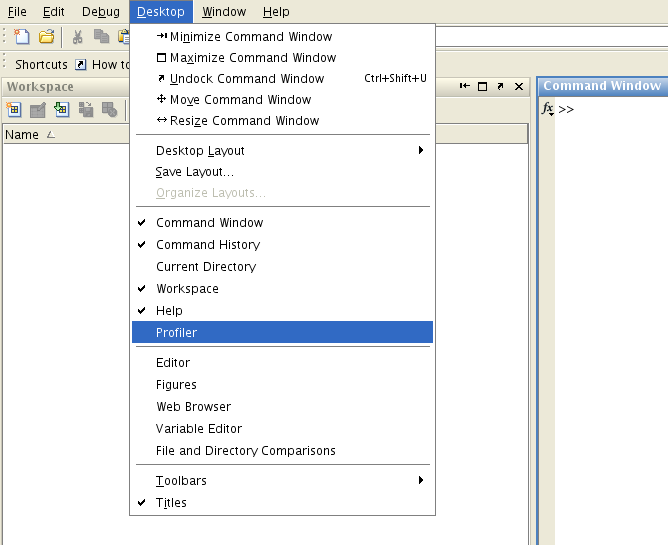
\includegraphics[height=5cm]{figures/matlab-open-profiler.png}}\\
\subfloat[][Part of the profiler output when running the routine of section on magic numbers (see page \pageref{example:magic-numbers}) one million times. Clearly, the \lstinline!norm! command takes longest to execute, so when trying to optimize one should start there.]{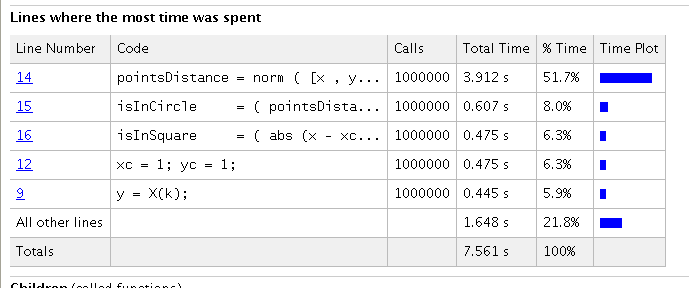
\includegraphics[height=5cm]{figures/matlab-profiler-circleBox-result.png}}
\caption{Using the profiler.}
\label{figure:profiler}
\end{figure}

\begin{remark}
Besides the graphical interface, there is also a command line version of the profiler that can be used to integrate it into your scripts. The commands to invoke are \lstinline!profile on! for starting the profiler and \lstinline!profile off! for stopping it, followed by various commands to evaluate the gathers statistics. See the \matlab{} help page on \lstinline!profile!.
\end{remark}


\subsection{The MATtrix LABoratory}

Contrary to common belief, the MAT in \matlab{} doesn't stand for mathematics, but \emph{matrix}. The reason for that is that proper \matlab{} code uses matrix and vector structures as often as possible, prominently at places where higher programming languages such as C of Fortran would rather use loops.

The reason for that lies in \matlab{}'s being an interpreted language. That means: There is no need for explicitly compiling the code, you just write it and have in run. The \matlab{} interpreter then scans your code line by line and executes the commands. As you might already suspect, this approach will never be able to compete with compiled source code.

However, \matlab{}'s internals contain certain precompiled functions which execute basic matrix-vector operations. Whenever the \matlab{} interpreter bumps into a matrix-vector expression, the contents of the matrices are forwarded to the underlying optimized and compiled code which, after execution, returns the result. This approach makes sure that matrix operations in \matlab{} are on par with matrix operations with compiled languages.

\begin{remark}
Not only for matrix-vector operations, precompiled binaries are provided. Most standard tasks in numerical linear algebra are handled with a customized version of the ATLAS (BLAS) library. This concerns for example commands such as \lstinline!eig()! (for finding the eigenvalues of a matrix), \lstinline!\! (for solving a linear equation system with Gau{\ss}ian\footnote{Johann Carl Friedrich Gau{\ss} (1777--1855), German mathematician and deemed one of the greatest mathematicians of all times. In the English-speaking world, the spelling with `ss' instead of the original `\ss' has achieved wide acceptance -- probably because the `\ss' is not included in the key set of any keyboard layout except the German one.} elimination), and so on.
\end{remark}

\subsubsection{Matrix pre-allocation -- \fastsymbol\fastsymbol\fastsymbol\fastsymbol\fastsymbol}

When a matrix appears in \matlab{} code for the first time, its contents need to be stored in system memory (RAM). This process is called allocation. To do this, \matlab{} needs to find a place in memory (a range of \emph{addresses}) which is large enough to hold the matrix and assign this place to the matrix. This process is called allocation. Note that typically, matrices are stored continuously in memory, and not split up to here and there. This way, the processor can quickly access its entries without having to look around in the system memory.

%  In some higher programming languages, the user needs to explicitly demand space allocation for an object, while in others do this automatically.

Now, what happens if the vector \lstinline!v! gets allocated with $55$ elements by, for example, \lstinline!v=rand(55,1)!, and the user decides later in the code to make it a little bigger, say, \lstinline!v=rand(1100,1)!? Well, obviously \matlab{} has to find a new slot in memory in case the old one is not wide enough to old all the new entries. This isn't so bad if it happens once or twice, but can slow down your code dramatically when a matrix is growing inside a loop, for example.


\hfill
\begin{minipage}[t]{.45\textwidth}
\begin{lstlisting}[framerule=2pt,rulecolor=\color{badred}]
n = 1e5;

for i = 1:n
    u(i) = sqrt(i);
end
\end{lstlisting}
The vector \lstinline!u! is growing \lstinline!n! times and it probably must be re-allocated as often. The approximate execution time of this code snippet is \extime{21.20}.
\end{minipage}
\hfill
\begin{minipage}[t]{.45\textwidth}
\begin{lstlisting}[framerule=2pt,rulecolor=\color{goodgreen}]
n = 1e5;
u = zeros(n,1);
for i = 1:n
    u(i) = sqrt(i);
end
\end{lstlisting}
As maximum size of the vector is known beforehand, one can easily tell \matlab{} to place \lstinline!u! into memory with the appropriate size. The code here merely takes \textbf{\SI{3.8}{\milli\second}} to execute!
\end{minipage}
\hfill

\begin{remark}
The previous code example is actually a little misleading as there is a much quicker way to fill \lstinline!u! with the square roots of consecutive numbers. Can you find the one-liner? A look into the next section could help\dots
\end{remark}


\subsubsection{Loop vectorization -- \fastsymbol\fastsymbol\fastsymbol\fastsymbol\fastsymbol}

Because of the reasons mentioned in the beginning of this section, you would like to avoid loops wherever you can and try to replace it by a vectorized operation.

When people commonly speak of `optimizing code for \matlab{}', it will most often be this particular aspect. The topic is huge and this section can merely give the idea of it. If you are stuck with slow loop operations and you have no idea how to make it really quick, take a look at the excellent and comprehensive guide at \cite{Mathworks:2009:CVG}. -- There is almost always a way to vectorize.

Consider the following example a general scheme of how to remove loops from vectorizable operations.

\hfill
\begin{minipage}[t]{.45\textwidth}
\begin{lstlisting}[framerule=2pt,rulecolor=\color{badred}]
n = 1e7;
a = 1;
b = 2;

x = zeros( n, 1 );
y = zeros( n, 1 );
for i=1:n
  x(i) = a + (b-a)/(n-1) ...
             * (i-1);
  y(i) = x(i) - sin(x(i))^2;
end
\end{lstlisting}
Computation of $f(x)=x-\sin^2(x)$ on \lstinline!n! points between \lstinline!a! and \lstinline!b!. In this version, each and every single point is being treated explicitly. Execution time: approx. \extime{0.91}.
\end{minipage}
\hfill
\begin{minipage}[t]{.45\textwidth}
\begin{lstlisting}[framerule=2pt,rulecolor=\color{goodgreen}]
n = 1e7;
a = 1;
b = 2;

h = 1/(n-1);


x = (a:h:b);

y = x - sin(x).^2;

\end{lstlisting}
Does the same thing using vector notation. Execution time: approx. \extime{0.12}.
\end{minipage}
\hfill

The \lstinline!sin()! function in \matlab{} hence takes a vector as argument and acts as of it operated on each element of it. Almost all \matlab{} functions have this capability, so make use of it if you can!


\paragraph{Vector indexing and boolean indexing.}\label{sec:logicalIndexing}
When dealing with vectors or matrices, it may sometimes happen that one has to work only on certain entries of the object, e.g., those with odd index.

Consider the following three different possibilties of setting the \emph{odd} entries of a vector \lstinline!v! to $0$.

\hfill
\begin{minipage}[t]{.29\textwidth}
\begin{lstlisting}[framerule=1pt,rulecolor=\color{goodgreen}]
% [...] create v

n = length(v);

for k = 1:2:n
  v(k) = 0;
end
\end{lstlisting}
Classical loop of the entries of interest (\extime{1.04}).
\end{minipage}
\hfill
\begin{minipage}[t]{.29\textwidth}
\begin{lstlisting}[framerule=1pt,rulecolor=\color{mediocre}]
% [...] create v

n = length(v);


v(1:2:n) = 0;

\end{lstlisting}
Vector indexing: Matrices take (positive) integer vectors as arguments (\extime{1.14}).
\end{minipage}
\hfill
\begin{minipage}[t]{.29\textwidth}
\begin{lstlisting}[framerule=1pt,rulecolor=\color{badred}]
% [...] create v

n = length(v);
mask = false(n,1);
mask(1:2:n) =true;
v( mask ) = 0;

\end{lstlisting}
Boolean indexing: Matrices take \emph{boolean} arrays\footnotemark{} with the same shape as \lstinline!v! as arguments (\extime{1.41}).
\end{minipage}
\hfill
\footnotetext{A mistake that beginners tend to make is to define \lstinline!mask! as an array of integers, such as \lstinline!mask = zeros(n,1);!.}

In this case, where the indices to be worked on are known beforehand, the classical way of looping over the error is the fastest. Vector indexing makes the code shorter, but creates a slight overhead; boolean indexing, by having to create the boolean array \lstinline!mask!, is significantly slower.

However, should the criteria upon which action is taken dynamically depend on the content of the vector itself, the situation is different.
Consider again the three schemes, this time for setting the \lstinline!NaN! entries of a vector \lstinline!v! to $0$.

\hfill
\begin{minipage}[t]{.29\textwidth}
\begin{lstlisting}[framerule=1pt,rulecolor=\color{badred}]
% [...] create v

for k = 1:n
  if isnan(v(k))
    v(k) = 0;
  end
end
\end{lstlisting}
Classical loop: \extime{1.19}.
\end{minipage}
\hfill
\begin{minipage}[t]{.29\textwidth}
\begin{lstlisting}[framerule=1pt,rulecolor=\color{mediocre}]
% [...] create v

ind = ...
  find(isnan(v));
v( ind ) = 0;


\end{lstlisting}
Vector indexing: \extime{0.44}.
\end{minipage}
\hfill
\begin{minipage}[t]{.29\textwidth}
\begin{lstlisting}[framerule=1pt,rulecolor=\color{goodgreen}]
% [...] create v

mask = isnan(v);

v( mask ) = 0;


\end{lstlisting}
Boolean indexing: \extime{0.33}.
\end{minipage}
\hfill

Iterating through the array \lstinline!v! and checking each element individually means disregarding the ``MAT'' in \matlab{}. Making use of the \lstinline!find()! function, it is possible to have \lstinline!isnan()! work on the whole vector before setting the desired indices to 0 in one go. Even better than that, doing away with the overhead that \lstinline!find()! creates, is to use the boolean array that \lstinline!isnan()! returns to index \lstinline!v! directly\footnote{Remember: You can combine several \lstinline!mask!s with the logical operators \lstinline!&! (``and'') and \lstinline!|! (``or''). For example, \lstinline!mask = isnan(v) | isinf(v);! is \lstinline!true! wherever \lstinline!v! has a \lstinline!NaN! \emph{or} an \lstinline!Inf!.}.


See also \cite{Mathworks:2001:MIM}.

% \begin{remark}
% Of course, things can get somewhat more difficult to vectorize, for example when the commands within the loop make contain more than just `\lstinline!i!' or `\lstinline!i-1!' as index references like above. There is, however, almost always a way to vectorize. If you don't know further, see \cite{Mathworks:2009:CVG}.
% \end{remark}

% \begin{example}
% The task is to write a function that gets a vector \lstinline!u! as input which contains
% \end{example}

% \subsubsection{Referencing matrix elements}
% This hint is actually pretty similar to what is stated in the previous paragraph.
% 
% One is sometimes confronted with the 
% 
% \Pointinghand\quad Useful functions: \lstinline!find!


\subsection{Solving a linear equation system -- \cleansymbol\cleansymbol\fastsymbol\fastsymbol\fastsymbol}
When being confronted with a standard linear equation system of the form $Au=b$, the solution can be written down as $u = A^{-1}b$ if $A$ is regular. It may now be quite seductive to translate this into \lstinline!u = inv(A)*b! in \matlab{} notation. Though this step will certainly yield the correct solution (neglecting round-off errors, which admittedly can be quite large in certain cases), it would take quite a long time to execute. The reason for this is the fact that the computer actually does more work then required. What you tell \matlab{} to do here is to
\begin{enumerate}
\item explicitly calculate the inverse of \lstinline!A!, store it in a temporary matrix, and then
\item multiply the this matrix with \lstinline!u!.
\end{enumerate}
However, one is most often not interested in the explicit form of $A^{-1}$, but only the final result $A^{-1}b$. The proper way out is \matlab{}'s \lstinline!\! (backslash) operator (or equivalently \lstinline!mldivide()!) which exactly serves the purpose of solving an equation system with Gau{\ss}ian elimination.

% While computing a full inverse takes $O(n^4)$ operations (with $n$ being the dimension of the matrix), solving the equation system is as expensive as $O(n^3)$, so you definitely want to go with it.

\hfill
\begin{minipage}[t]{.45\textwidth}
\begin{lstlisting}[framerule=2pt,rulecolor=\color{badred}]
n = 2e3;
A = rand(n,n);
b = rand(n,1);

u = inv(A)*b;
\end{lstlisting}
Solving the equation system with an explicit inverse. Execution time: approx. \extime{2.02}.
\end{minipage}
\hfill
\begin{minipage}[t]{.45\textwidth}
\begin{lstlisting}[framerule=2pt,rulecolor=\color{goodgreen}]
n = 2e3;
A = rand(n,n);
b = rand(n,1);

u = A\b;
\end{lstlisting}
Solving the equation system with the \lstinline!\! operator. Execution time: approx. \extime{0.80}.
\end{minipage}
\hfill

% The speed gain is actually not as ground-breaking as the order of magnitude points to; this suggests that \matlab{} actually has some build-in logic that works around this user's mistake. Still, using \lstinline!inv()! for solving an equation system in \matlab{} is considered a deadly sin in \matlab{} and should under all circumstances be avoided.


\subsection{Dense and sparse matrices -- \fastsymbol\fastsymbol\fastsymbol\fastsymbol\fastsymbol}

Most discretizations of particular problems yield $N\times N$-matrices which only have a small number of non-zero elements (proportional to $N$). These are called sparse matrices, and as they appear so very often, there is plenty of literature describing how to make use of that structure.

In particular, one can
\begin{itemize}
\item cut down the amount of memory used to store the matrix. Of course, instead of storing all the $0$'s, one would rather store the value and indices of the non-zero elements in the matrix. There are different ways of doing so. \matlab{} internally uses the condensed-column format, and exposes the matrix to the user in indexed format.

\item optimize algorithms for the use with sparse matrices. As a matter of fact, most basic numerical operations (such as Gau{\ss}ian elimination, eigenvalue methods and so forth) can be reformulated for sparse matrices and save an enormous amount of computational time.
\end{itemize}

% For these reasons, it is highly recommended to allocate matrices as sparse when they really are. There are a couple of functions which assist building up a sparse matrix, most notably \lstinline!sparse!, \lstinline!spdiags!, and \lstinline!speye!.

Of course, operations which only involve sparse matrices will also return a sparse matrix (such as matrix--matrix multiplication \lstinline!*!, \lstinline!transpose!, \lstinline!kron!, and so forth).



\hfill
\begin{minipage}[t]{.45\textwidth}
\begin{lstlisting}[framerule=2pt,rulecolor=\color{badred}]
n = 1e4;
h = 1/(n+1);

A = zeros(n,n);
A(1,1) =  2;
A(1,2) = -1;
for i=2:n-1
    A(i,i-1) = -1;
    A(i,i  ) =  2;
    A(i,i+1) = -1;
end
A(n,n-1) = -1;
A(n,n)   =  2;

A = A / h^2;

% continued below
\end{lstlisting}
Creating the tridiagonal matrix $1/h^2\times\diag[-1, 2, -1]$ in dense format. The code is bulky for what it does, and can't use native matrix notation. Execution time: \extime{0.67}.
\end{minipage}
\hfill
\begin{minipage}[t]{.45\textwidth}
\begin{lstlisting}[framerule=2pt,rulecolor=\color{goodgreen}]
n = 1e4;
h = 1/(n+1);

e = ones(n,1);
A = spdiags([-e 2*e -e],...
            [-1   0  1],...
             n, n );







A = A / h^2;

% continued below
\end{lstlisting}
The three-line equivalent using the sparse matrix format. The code is not only shorter, easier to read, but also saves gigantic amounts of memory. Execution time: \textbf{\SI{5.4}{\milli\second}}!
\end{minipage}
\hfill

\medskip

\hfill
\begin{minipage}[t]{.45\textwidth}
\begin{lstlisting}[framerule=2pt,rulecolor=\color{badred}]
% A in dense format
b = ones(n,1);
u = A\b;
\end{lstlisting}
Gau{\ss}ian elimination with a tridiagonal matrix in dense format. Execution time: \extime{55.06}.
\end{minipage}
\hfill
\begin{minipage}[t]{.45\textwidth}
\begin{lstlisting}[framerule=2pt,rulecolor=\color{goodgreen}]
% A in sparse format
b = ones(n,1);
u = A\b;
\end{lstlisting}
The same syntax, with \lstinline!A! being sparse. Execution time: \textbf{\SI{0.36}{\milli\second}}!
\end{minipage}
\hfill

% \begin{remark}
% Of course, not all matrices are sparse.
% \end{remark}

\Pointinghand\hspace{1em} Useful functions: \lstinline!sparse()!, \lstinline!spdiags()!, \lstinline!speye()!, (\lstinline!kron()!),\dots



\subsection{Repeated solution of an equation system with the same matrix -- \fastsymbol\fastsymbol\fastsymbol\fastsymbol\fastsymbol}

It might happen sometimes that you need to solve an equation system a number of times with the same matrix but different right-hand sides. When all the right hand sides are immediately available, this can be achieved with with one ordinary `\lstinline!\!' operation.

\hfill
\begin{minipage}[t]{.45\textwidth}
\begin{lstlisting}[framerule=2pt,rulecolor=\color{badred}]
n = 1e3;
k = 50;
A = rand(n,n);
B = rand(n,k);

u = zeros(n,k);

for i=1:k
    u(:,k) = A \ B(:,k);
end
\end{lstlisting}
Consecutively solving with a couple of right-hand sides. Execution time: \extime{5.64}.
\end{minipage}
\hfill
\begin{minipage}[t]{.45\textwidth}
\begin{lstlisting}[framerule=2pt,rulecolor=\color{goodgreen}]
n = 1e3;
k = 50;
A = rand(n,n);
B = rand(n,k);




u = A \ B;

\end{lstlisting}
Solving with a number of right hand sides in one go. Execution time: \extime{0.13}.
\end{minipage}
\hfill


If, on the other hand, you need to solve the system once to get the next right-hand side (which is often the case with time-dependent differential equations, for example), this approach won't work; you'll indeed have to solve the system in a loop. However, one would still want to use the information from the previous steps; this can be done by first factoring $A$ into a product of a lower triangular matrix $L$ and an upper triangular matrix $U$, and then instead of computing $A^{-1}u^{(k)}$ in each step, computing $U^{-1}L^{-1}u^{(k)}$ (which is a lot cheaper.

\hfill
\begin{minipage}[t]{.45\textwidth}
\begin{lstlisting}[framerule=2pt,rulecolor=\color{badred}]
n = 2e3;
k = 50;
A = rand(n,n);

u = ones(n,1);


for i = 1:k
  u = A\u;
end
\end{lstlisting}
Computing $u = A^{-k}u_0$ by solving the equation systems in the ordinary way. Execution time: \extime{38.94}.
\end{minipage}
\hfill
\begin{minipage}[t]{.45\textwidth}
\begin{lstlisting}[framerule=2pt,rulecolor=\color{goodgreen}]
n = 2e3;
k = 50;
A = rand(n,n);

u = ones(n,1);

[L,U] = lu( A );
for i = 1:k
  u = U\( L\u );
end
\end{lstlisting}
Computing $u = A^{-k}u_0$ by $LU$-factoring the matrix, then solving with the $LU$ factors. Execution time: \extime{5.35}. Of course, when increasing  the number $k$ of iterations, the speed gain compared to the `\lstinline!A\!' will  be more and more dramatic.
\end{minipage}
\hfill

\begin{remark}
For many matrices $A$ in the above example, the final result will be heavily corrupted with round-off errors such that after $k=50$ steps, the norm of the residual $\norm{u_0-A^ku}$, which ideally equals $0$, can be pretty large.
\end{remark}


\paragraph{Factorizing sparse matrices.}
When $LU$- or Cholesky-factorizing a \emph{sparse matrix}, the factor(s) are in general not sparse anymore and can demand quite an amount of space in memory to the point where no computer can cope with that anymore. The phenomenon of having non-zero entries in the $LU$- or Cholesky-factors where the orginal matrix had zeros is called \emph{fill-in} and has attracted a lot of attention in the past 50 years. As a matter of fact, the success of iterative methods for solving linear equation systems is largely thanks to this drawback.

Beyond using an iterative method to solve the system, the most popular way to cope with fill-in is to try to re-order the matrix elements in such a way that the new matrix induces less fill-in. Examples of re-ordering are \emph{Reverse Cuthill-McKee} and \emph{Approximate Minimun Degree}. Both are implemented in \matlab{} as \lstinline!colrcm()! and \lstinline!colamd()!, respectively (with versions \lstinline!symrcm()! and \lstinline!symamd()! for symmetric matrices).

One can also leave all the fine-tuning to \matlab{} by executing \lstinline!lu()! for sparse matrices with more output arguments; this will return a factorization for the permuted and row-scaled  matrix $PR^{-1}AQ = LU$ (see \matlab{}'s help pages and example below) to reduce fill-in and increase the stability of the algorithm.

\hfill
\begin{minipage}[t]{.45\textwidth}
\begin{lstlisting}[framerule=2pt,rulecolor=\color{badred}]
n = 2e3;
k = 50;

% get a non-singular nxn
% sparse matrix A:
% [...]

u = ones(n,1);

[L,U] = lu( A );
for i = 1:k
  u = U\( L\u );
end
\end{lstlisting}
Ordinary $LU$-factorization for a sparse matrix \lstinline!A!. The factors \lstinline!L! and \lstinline!U! are initialized as sparse matrices as well, but the fill-in phenomenon will undo this advantage. Execution time: \extime{4.31}.
\end{minipage}
\hfill
\begin{minipage}[t]{.45\textwidth}
\begin{lstlisting}[framerule=2pt,rulecolor=\color{goodgreen}]
n = 2e3;
k = 50;

% get a non-singular nxn
% sparse matrix A:
% [...]

u = ones(n,1);

[L,U,P,Q,R] = lu(A);
for i = 1:k
  u = Q*( U\(L\(P*(R\u))) );
end
\end{lstlisting}
$LU$-factoring with permutation and row-scaling. This version can use less memory, execute faster, and provide more stability than the ordinary $LU$-factorization. Execution time: \extime{0.07}.

This factorization is implicitly applied by \matlab{} when using the `\lstinline!\!'-operator for solving a sparse system of equations \emph{once}.
\end{minipage}
\hfill

% =============================================================================
%
% Copyright (c) 2009--2013, Nico Schlömer
% All rights reserved.
%
% Redistribution and use in source and binary forms, with or without
% modification, are permitted provided that the following conditions are
% met:
%
%     * Redistributions of source code must retain the above copyright
%       notice, this list of conditions and the following disclaimer.
%     * Redistributions in binary form must reproduce the above copyright
%       notice, this list of conditions and the following disclaimer in
%       the documentation and/or other materials provided with the distribution
%
% THIS SOFTWARE IS PROVIDED BY THE COPYRIGHT HOLDERS AND CONTRIBUTORS "AS IS"
% AND ANY EXPRESS OR IMPLIED WARRANTIES, INCLUDING, BUT NOT LIMITED TO, THE
% IMPLIED WARRANTIES OF MERCHANTABILITY AND FITNESS FOR A PARTICULAR PURPOSE
% ARE DISCLAIMED. IN NO EVENT SHALL THE COPYRIGHT OWNER OR CONTRIBUTORS BE
% LIABLE FOR ANY DIRECT, INDIRECT, INCIDENTAL, SPECIAL, EXEMPLARY, OR
% CONSEQUENTIAL DAMAGES (INCLUDING, BUT NOT LIMITED TO, PROCUREMENT OF
% SUBSTITUTE GOODS OR SERVICES; LOSS OF USE, DATA, OR PROFITS; OR BUSINESS
% INTERRUPTION) HOWEVER CAUSED AND ON ANY THEORY OF LIABILITY, WHETHER IN
% CONTRACT, STRICT LIABILITY, OR TORT (INCLUDING NEGLIGENCE OR OTHERWISE)
% ARISING IN ANY WAY OUT OF THE USE OF THIS SOFTWARE, EVEN IF ADVISED OF THE
% POSSIBILITY OF SUCH DAMAGE.
%
% =============================================================================
\newpage
\section{Other tips \& tricks}

% \begin{listing}
% \begin{minted}[frame=single,framerule=2pt,color=\color{badred}]{matlab}
% % ===================================================
% % *** FUNCTION simpson
% % ***
% % *** Implements Simpson's rule for integrating
% % *** the sine function over [a,b] with granularity
% % *** h.
% % ***
% % ===================================================
% function int = simpson( a, b, h )
%
%   x = a:h:b;
%
%   int = 0;
%   n   = length(x);
%   mid = (x(1:n-1) + x(2:n)) / 2;
%   int = sum( h/6 * (    sin(x(1:n-1)) ...
%                     + 4*sin(mid     ) ...
%                     +   sin(x(2:n  )) ) );
%
% end
% % ===================================================
% % *** END FUNCTION simpson
% % ===================================================
% \end{minted}
% \caption{Implementation of Simpson's rule for numerically integrating a function (here: \lstinline!sin!) between \lstinline!a! and \lstinline!b!. Note the usage of the vector notation to speed up the function. Also note that \lstinline!sin! is hardcoded into the routine, and needs to be changed each time we want to change the function. In case one is interested in calculating the integral of $f(x) = \exp(\sin(\frac{1}{x})) / \tan(\sqrt{1-x^4})$, this could get quite messy.}
% \label{listing:simpson1}
% \end{listing}


\begin{lstlisting}[
framerule=2pt,
float,
label={listing:simpson1},
caption={Implementation of Simpson's rule for numerically integrating a function (here: \lstinline!sin!) between \lstinline!a! and \lstinline!b!. Note the usage of the vector notation to speed up the function. Also note that \lstinline!sin! is hardcoded into the routine, and needs to be changed each time we want to change the function. In case one is interested in calculating the integral of $f(x) = \exp(\sin(\frac{1}{x})) / \tan(\sqrt{1-x^4})$, this could get quite messy.},
rulecolor=\color{badred}]
% ===================================================
% *** FUNCTION simpson
% ***
% *** Implements Simpson's rule for integrating
% *** the sine function over [a,b] with granularity
% *** h.
% ***
% ===================================================
function int = simpson( a, b, h )

  x = a:h:b;

  int = 0;
  n   = length(x);
  mid = (x(1:n-1) + x(2:n)) / 2;
  int = sum( h/6 * (    sin(x(1:n-1)) ...
                    + 4*sin(mid     ) ...
                    +   sin(x(2:n  )) ) );

end
% ===================================================
% *** END FUNCTION simpson
% ===================================================
\end{lstlisting}

\subsection{Functions as arguments -- \cleansymbol\cleansymbol\cleansymbol}

In numerical computation, there are set-ups which natively treat functions as
the objects of interest, for example when numerically integrating them over a
particular domain. For this example, imagine that you wrote a function that
implements Simpson's integration rule (see listing~\ref{listing:simpson1}),
and you would like to apply it to a number of functions without having to
alter your source code (for example, replacing \lstinline!sin()! by
\lstinline!cos()!, \lstinline!exp()! or something else).

A clean way to deal with this in \matlab{} is using \emph{function handles}. This may sound fancy, and describes nothing else then the capability of treating functions (such as \lstinline!sin()!) as arguments to other functions (such as \lstinline!simpson()!). The function call itself is written as easy as

\begin{lstlisting}[
float,
caption={Simpson's rule with function handles. Note that the syntax for function arguments is no different from that of ordinary ones.},
label={listing:simpson2},
framerule=2pt,
rulecolor=\color{goodgreen}]
% ===================================================
% *** FUNCTION simpson
% ***
% *** Implements Simpson's rule for integrating
% *** a function f over [a,b] with granularity h.
% ***
% ===================================================
function int = simpson( f, a, b, h )

  x   = a:h:b;
  mid = (x(1:n-1) + x(2:n)) / 2;

  n   = length(x);

  int = sum( h/6 * (    f(x(1:n-1)) ...
                    + 4*f(mid     ) ...
                    +   f(x(2:n  )) ) );

end
% ===================================================
% *** END FUNCTION simpson
% ===================================================
\end{lstlisting}

\hfill
\begin{minipage}[t]{.90\textwidth}
\begin{lstlisting}[framerule=1pt,rulecolor=\color{goodgreen}]
a = 0;
b = pi/2;
h = 1e-2;
int_sin = simpson( @sin, a, b, h );
int_cos = simpson( @cos, a, b, h );
int_f   = simpson( @f  , a, b, h );
\end{lstlisting}
\end{minipage}
\hfill

where the function name need to be prepended by the `\lstinline!@!'-character.

The function \lstinline!f()! can be any function that you defined yourself and
which is callable as \lstinline!f(x)! with \lstinline!x! being a vector of $x$
values (like it is used in \lstinline!simpson()!, listing~\ref{listing:simpson2}).



\subsection{Implicit matrix--vector products -- \cleansymbol}

In numerical analysis, almost all methods for solving linear equation systems
\emph{quickly} are iterative methods, that is, methods which define how to
iteratively approach a solution in small steps (starting with some initial
guess) rather then directly solving them in one big step (such as Gau{\ss}ian
elimination). Two of the most prominent iterative methods are CG and GMRES.

In particular, those methods \emph{do not require the explicit availability of
the matrix} as in each step of the iteration they merely form a matrix-vector
product with $A$ (or variations of it). Hence, they technically only need a
function to tell them how to carry out a matrix-vector multiplication. In some
cases, providing such a function may be easier than explicitly constructing
the matrix itself, as the latter usually requires one to pay close attention
to indices (which can get extremely messy).

Beyond that, there may also a mild advantage in memory consumption as the
indices of the matrix do no longer need to sit in memory, but can be hard coded
into the matrix-vector-multiplication function itself. Considering the fact
that we are mostly working with sparse matrices however, this might not be
quite important.

The example below illustrates the typical benefits and drawbacks of the
approach.

\begin{lstlisting}[
float,
framerule=1pt,
caption={Function that implements matrix--vector multiplication with $1/h^2 \times \diag(-1,2,-1)$. Note that the function consumes (almost) no more memory then \lstinline!u! already required.},
label={listing:Amultiply}
]
% ===================================================
% *** FUNCTION A_multiply
% ***
% *** Implements matrix--vector multiplication with
% *** diag[-1,2,-1]/h^2  .
% ***
% ===================================================
function out = A_multiply( u )

  n   = length( u );
  u   = [0; u; 0];

  out = -u(1:n) + 2*u(2:n+1) - u(3:n+2);
  out = out * (n+1)^2;

end
% ===================================================
% *** END FUNCTION A_multiply
% ===================================================
\end{lstlisting}


\hfill
\begin{minipage}[t]{.45\textwidth}
\begin{lstlisting}[framerule=1pt]
n = 1e3;
k = 500;







u = ones(n,1);
for i=1:k
    u = A_multiply( u );
end
\end{lstlisting}
Computing $u = A^ku_0$ with the function \lstinline!A_multiply!
(listing~\ref{listing:Amultiply}). The memory consumption of this routine is
(almost) no greater than storing $n$ real numbers. Execution time:
\extime{21}.
\end{minipage}
\hfill
\begin{minipage}[t]{.45\textwidth}
\begin{lstlisting}[framerule=1pt]
n = 1e3;
k = 500;

e = ones(n,1);
A = spdiags([-e,2*e,-e],...
            [-1,  0,-1],...
             n, n );
A = A * (n+1)^2;

u = ones(n,1);
for i=1:k
    u = A*u;
end
\end{lstlisting}
Computing $u = A^ku_0$ with a regular sparse format matrix \lstinline!A!, with the need to store it in memory. Execution time: \extime{7}.
\end{minipage}
\hfill

All in all, these considerations shall not lead you to rewrite all you
matrix-vector multiplications as function calls. Mind, however, that there are
situations where one would \emph{never} use matrices in their explicit form,
although mathematically written down like that:

\begin{example}[Multigrid]
In geometric multigrid methods, a domain is discretized with a certain
parameter $h$ (``grid width'') and the operator $A_h$ written down for that
discretization (see the examples above, where $A_h=h^{-2}\diag(-1,2,1)$ is
really the discretization of the $\Delta$-operator in one dimension). In a
second step, another, somewhat coarser grid is considered with $H=2h$, for
example. The operator $A_H$ on the coarser grid is written down as
\[
A_H = I_h^H A_h I_H^h,
\]
where the $I_*^*$ operators define the transition from the coarse to the fine
grid, or the other way around. When applying it to a vector on the coarse grid
$u_H$ ($A_Hu_H =I_h^H A_h I_H^h u_H$), the above definition reads:
\begin{enumerate}
\item $I_H^h u_H$: Map $u_H$ to the fine grid.
\item $A_h\cdot$: Apply the fine grid operator to the transformation.
\item $I_h^H\cdot$: Transform the result back to the coarse grid.
\end{enumerate}
How the transformations are executed needs to be defined. One could, for
example, demand that $I_H^h$ maps all points that are part of the fine grid
\emph{and} the coarse grid to itself; all points on the fine grid, that lie
right in between two coarse variables get half of the value of each of the two
(see figure~\ref{subfig:coarse-fine}).

\begin{figure}
\centering
\begin{subfigure}{0.45\textwidth}
  \begin{tikzpicture}[node/.style={circle,draw=black!50,fill=black!10,thick,font=\footnotesize},scale=0.7,
arrownote/.style={black,font=\footnotesize}]


\node (u1) at (0,3) [node] {$u_{H,1}$};
\node (u2) at (4,3) [node] {$u_{H,2}$};
\node (u3) at (8,3) [node] {$u_{H,3}$};


\node (u5) at (0,0) [node] {$u_{h,1}$};
\node (u6) at (2,0) [node] {$u_{h,2}$};
\node (u7) at (4,0) [node] {$u_{h,3}$};
\node (u8) at (6,0) [node] {$u_{h,4}$};
\node (u9) at (8,0) [node] {$u_{h,5}$};

\draw [very thick] (u1) -- (u2) --(u3);
\draw [very thick] (u5) --(u6) --(u7) --(u8) --(u9);

\draw [->,black!50] (u1) to node [arrownote,left] {$1$}  (u5) ;
\draw [->,black!50] (u1) to node [arrownote,right] {$\frac{1}{2}$} (u6) ;

\draw [->,black!50] (u2) to node [arrownote,left] {$\frac{1}{2}$} (u6) ;
\draw [->,black!50] (u2) to node [arrownote,right] {$1$} (u7) ;
\draw [->,black!50] (u2) to node [arrownote,right] {$\frac{1}{2}$} (u8) ;

\draw [->,black!50] (u3) to node [arrownote,left] {$\frac{1}{2}$} (u8) ;
\draw [->,black!50] (u3) to node [arrownote,right] {$1$} (u9) ;

\end{tikzpicture}
  \caption{Possible transformation rule when translating values from the
  coarse to the fine grid. See listing~\ref{listing:IHh}.}
  \label{subfig:coarse-fine}
\end{subfigure}
\hfill
\begin{subfigure}{0.45\textwidth}
  \begin{tikzpicture}[
node/.style={circle,draw=black!50,fill=black!10,thick,font=\footnotesize},scale=0.7,
arrownote/.style={black,font=\footnotesize}]

\node (u1) at (0,3) [node] {$u_{H,1}$};
\node (u2) at (4,3) [node] {$u_{H,2}$};
\node (u3) at (8,3) [node] {$u_{H,3}$};

\node (u5) at (0,0) [node] {$u_{h,1}$};
\node (u6) at (2,0) [node] {$u_{h,2}$};
\node (u7) at (4,0) [node] {$u_{h,3}$};
\node (u8) at (6,0) [node] {$u_{h,4}$};
\node (u9) at (8,0) [node] {$u_{h,5}$};

\draw [very thick] (u1) -- (u2) --(u3);blue
\draw [very thick] (u5) --(u6) --(u7) --(u8) --(u9);

\draw [->,black!50] (u5) to node [arrownote,left] {$\frac{1}{2}$}  (u1) ;
\draw [->,black!50] (u6) to node [arrownote,right] {$\frac{1}{4}$} (u1) ;

\draw [->,black!50] (u6) to node [arrownote,left] {$\frac{1}{4}$} (u2) ;
\draw [->,black!50] (u7) to node [arrownote,right] {$\frac{1}{2}$} (u2) ;
\draw [->,black!50] (u8) to node [arrownote,right] {$\frac{1}{4}$} (u2) ;

\draw [->,black!50] (u8) to node [arrownote,left] {$\frac{1}{4}$} (u3) ;
\draw [->,black!50] (u9) to node [arrownote,right] {$\frac{1}{2}$} (u3) ;

\end{tikzpicture}

  \caption{Mapping back from fine to coarse.}
  \label{subfig:fine-coarse}
\end{subfigure}
\caption{}
\end{figure}


\begin{lstlisting}[
float,
framerule=1pt,
caption={Function that implements the operator $I_H^h$ from the example (see figure~\ref{subfig:coarse-fine}). Writing down the structure of the corresponding matrix would be somewhat complicated, and even more so when moving to two- or three-dimensional grids. Note also how matrix notation has been exploited.},
label={listing:IHh}
]
% ===========================================================
% *** FUNCTION coarse2fine
% ***
% *** Transforms values from a coarse grid to a fine grid.
% ***
% ===========================================================
function uFine = coarse2fine( uCoarse )

  N = length(uCoarse);
  n = 2*N - 1;

  uFine(1:2:n) = uCoarse;

  midValues    = 0.5 * ( uCoarse(1:N-1) + uCoarse(2:N) );
  uFine(2:2:n) = midValues;

end
% ===========================================================
% *** END FUNCTION coarse2fine
% ===========================================================
\end{lstlisting}


In the analysis of the method, $I_H^h$ and $I_h^H$ will always be treated as
matrices, but when implementing, one would \emph{certainly not} try to figure
out the structure of the matrix. It is a lot simpler to implement a function
that executes the rule suggested above, for example.
\end{example}


\nocite{
Getreuer:2004:WFM,
Acklam:2003:MAM,
Moler:2004:NCM,
Moler:2008:EM}
\printbibliography

\end{document}